\documentclass{../document}

\addbibresource{refs.bib}

\newcommand{\Caltech}{Theoretical Astrophysics 350-17, California Institute of Technology, Pasadena, CA 91125, USA}
  \newcommand{\CaltechId}{1}
\newcommand{\Oberlin}{Department of Physics and Astronomy, Oberlin College, Oberlin, Ohio 44074, USA}
  \newcommand{\OberlinId}{2}
\newcommand{\Cornell}{Cornell Center for Astrophysics and Planetary Science, Cornell University, Ithaca, New York 14853, USA}
  \newcommand{\CornellId}{3}

\begin{document}
  \thispagestyle{plain}

  \vspace*{0.5cm}

  \begin{center}
    \Large\bf
    Control of Physical Parameters in \\
    Binary Black Hole Initial Data
  \end{center}
    
  \begin{center}
    Iago Mendes$^{\CaltechId,\OberlinId}$
      \orcidlink{0009-0007-9845-8448}
  \end{center}

  \begin{flushleft}
    Mentors:
      Nils Vu$^\CaltechId$
        \orcidlink{0000-0002-5767-3949},
      Mark Scheel$^\CaltechId$
        \orcidlink{0000-0001-6656-9134},
      Saul Teukolsky$^{\CaltechId,\CornellId}$
        \orcidlink{0000-0001-9765-4526}
  \end{flushleft}
   
  \begin{flushleft}
    \footnotesize
    $^\CaltechId$\Caltech \\
    $^\OberlinId$\Oberlin \\
    $^\CornellId$\Cornell
  \end{flushleft}

  \begin{flushleft}
    This report was submitted as part of the Summer Undergraduate Research Fellowship (SURF) program at Caltech.
  \end{flushleft}

  \begin{center}
    (Dated: \today)
  \end{center}

  \vspace*{0.5cm}

  \section*{Abstract}

    When solving Einstein's equations for Binary Black Holes (BBH) numerically, we split the four-dimensional spacetime into three-dimensional spatial slices and evolve them over time. The first slice is described by solving an Initial Data problem, which is cast as five elliptic partial differential equations in the extended conformal thin-sandwich (XCTS) decomposition. Prior to solving the XCTS equations, we must choose ``free data'' to impose boundary conditions and specify background quantities. This is the approach taken in {\tt SpECTRE}, a parallel code that aims to simulate BBH for the new generations of gravitational wave detectors. After solving the XCTS system, {\tt SpECTRE} runs a horizon finder that measures the masses and spins of the black holes. Additionally, our work extends {\tt SpECTRE}'s capabilities to calculate total energy, momentum, and center of mass as infinite integrals using the Arnowitt-Deser-Misner (ADM) formalism. Typically, we want to choose these physical quantities before running a BBH simulation, but they can only be measured after numerically solving the XCTS equations. To address this, we implemented an iterative scheme in {\tt SpECTRE} that drives the physical parameters to their desired values by adjusting the free data in a quasi-Newton-Raphson method that efficiently computes the Jacobian with Broyden's method.

  \section{Introduction}
    
    In the early twentieth century, Einstein revolutionized the study of gravity by connecting spacetime geometry with physical dynamics. As John Wheeler says, ``Spacetime tells matter how to move; matter tells spacetime how to curve'' \cite{Wheeler}. Being a highly complex theory, many problems of interest only have analytic solutions in special cases with symmetry. In this context, Numerical Relativity emerged as an essential field to solve these problems numerically, allowing us to explore general cases that can be found in the universe. Specifically, simulations of Binary Black Holes (BBH) became very important as gravitational wave detectors were developed, needing to use numerical results to identify and characterize signals in their data \cite{LIGO}.

    Famously, the Einstein equations relate the curvature of spacetime to the stress-energy of matter, forming a system of ten nonlinear partial differential equations (PDEs). With the 3+1 formalism, we can rearrange these equations so that spacetime is described by spacelike three-dimensional slices of constant time \cite{Alcubierre}. In doing so, we find that four out of the ten equations do not involve time derivatives, implying that they are constraints that must be satisfied at all times. The remaining six equations describe an evolution of the constraint-satisfying fields. Using this formalism, the Spectral Einstein Code ({\tt SpEC}) \cite{SpEC} runs BBH simulations by first finding initial data and then running an evolution on them. Over time, as {\tt SpEC} faced more challenging BBH with high mass ratios and spins, several improvements had to be made to the initial data techniques, which are summarized in \cite{Serguei}.
    
    Despite its success in BBH simulations, {\tt SpEC} shows its limitations in more challenging problems, such as binary neutron star mergers and BBH with extreme configurations. In this context, {\tt SpECTRE} \cite{SpECTRE} was created as a codebase that follows a better parallelism model and aims to be more scalable \cite{Kidder}. Previous work has already shown that {\tt SpECTRE} can be faster and more accurate than {\tt SpEC} when performing similar tasks due to its use of parallelism \cite{Vu}. This will be especially needed for the upcoming gravitational wave detectors with higher sensitivity, such as the Cosmic Explorer, the Einstein Telescope and LISA.
    
    As part of an effort to allow researchers to fully simulate BBH in {\tt SpECTRE}, an initial data procedure similar to the one in {\tt SpEC} needs to be completed. This is greatly benefitted by a scalable elliptic solver that was recently developed \cite{Vu}, which can now be used to solve the initial data equations. Be that as it may, before the start of the SURF program, {\tt SpECTRE} did not have a way to enforce specific masses and spins for the black holes or to avoid drifts in their orbital trajectories. This report describes how we addressed these issues.

    In section...

  \section{Theory}

    \subsection{The XCTS system}

      To find initial data, {\tt SpECTRE} uses the extended conformal thin-sandwich (XCTS) decomposition, which casts Einstein's equations as a system of five elliptic PDEs:
      

    \subsection{Calculation of asymptotic quantities}

  \section{Numerical method}
  
  \section{Results}

    \subsection{Convergence of asymptotic quantities}

      \begin{figure}
        \centering
        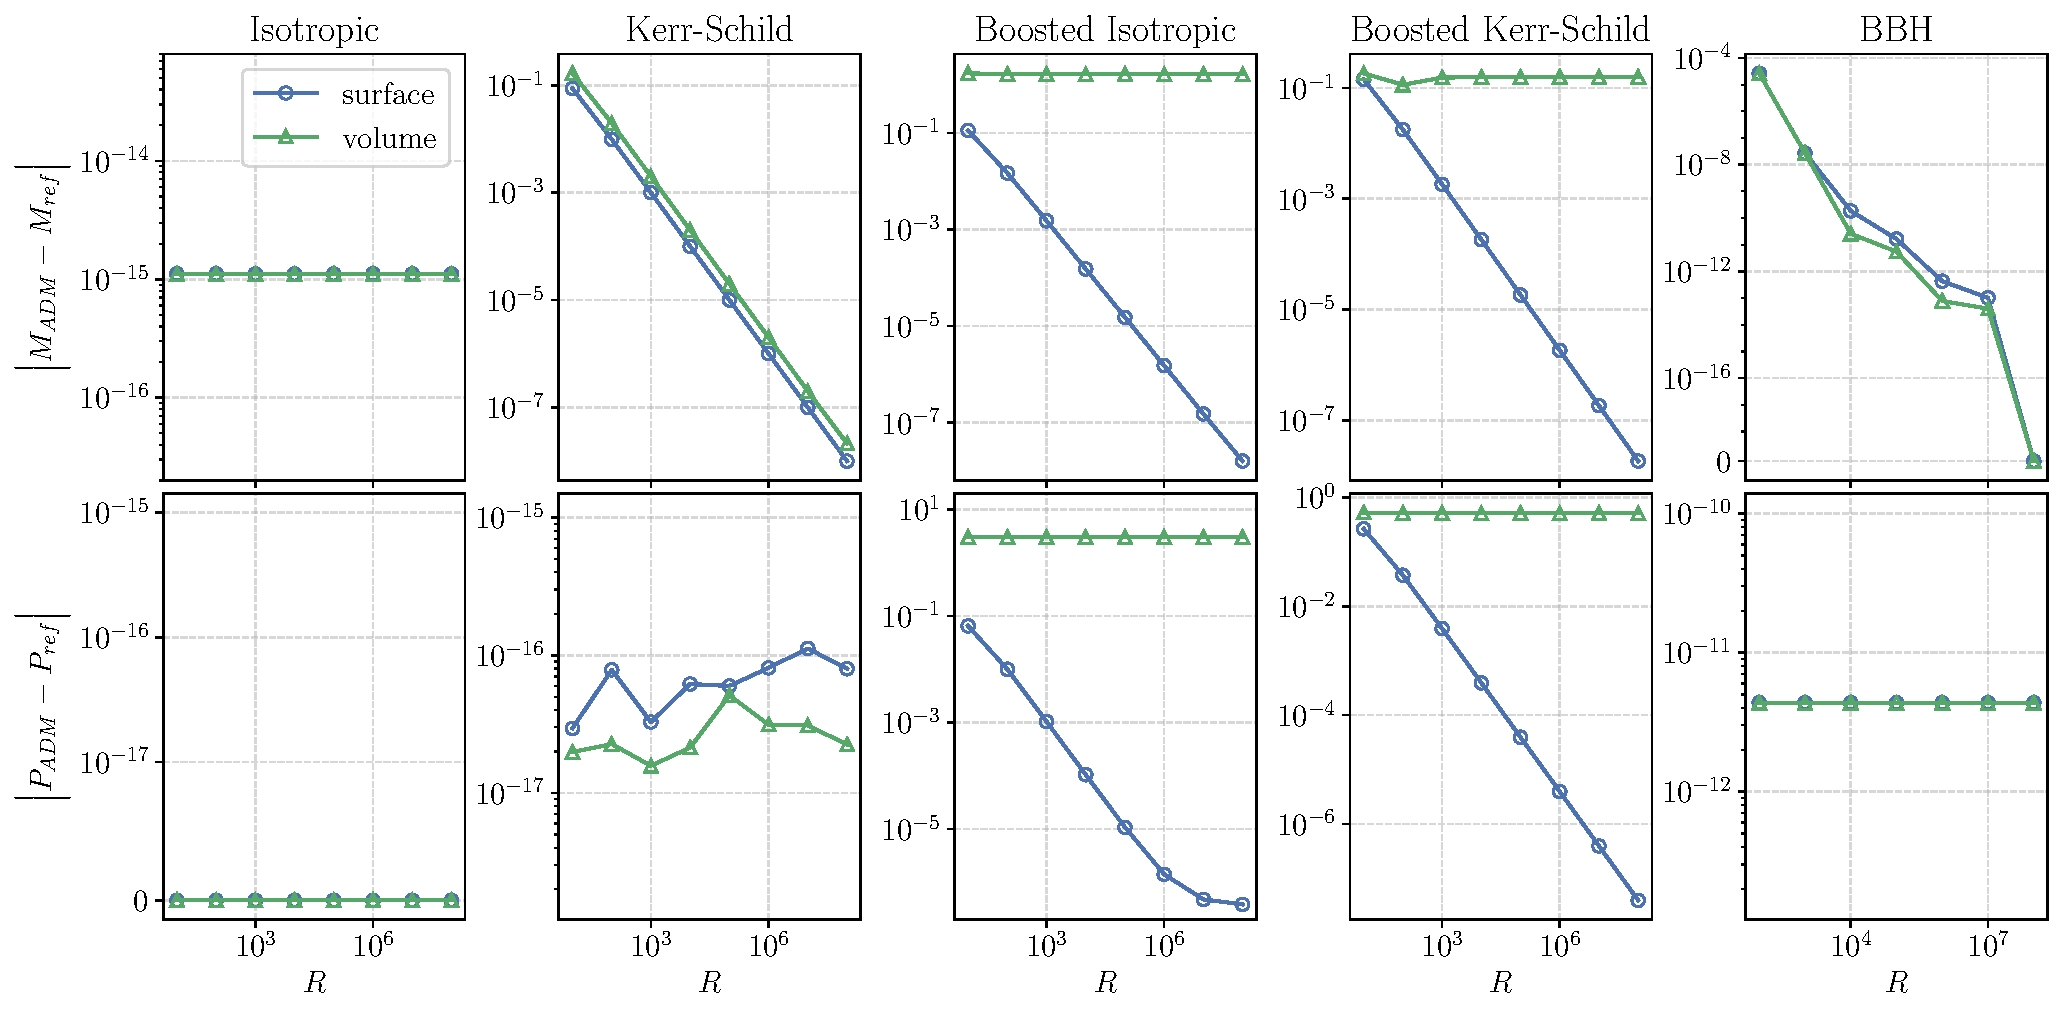
\includegraphics[width=\textwidth]{../../plots/final_report/distance_convergence_Madm_Padm.pdf}
        \caption{}
      \end{figure}

      \begin{figure}
        \centering
        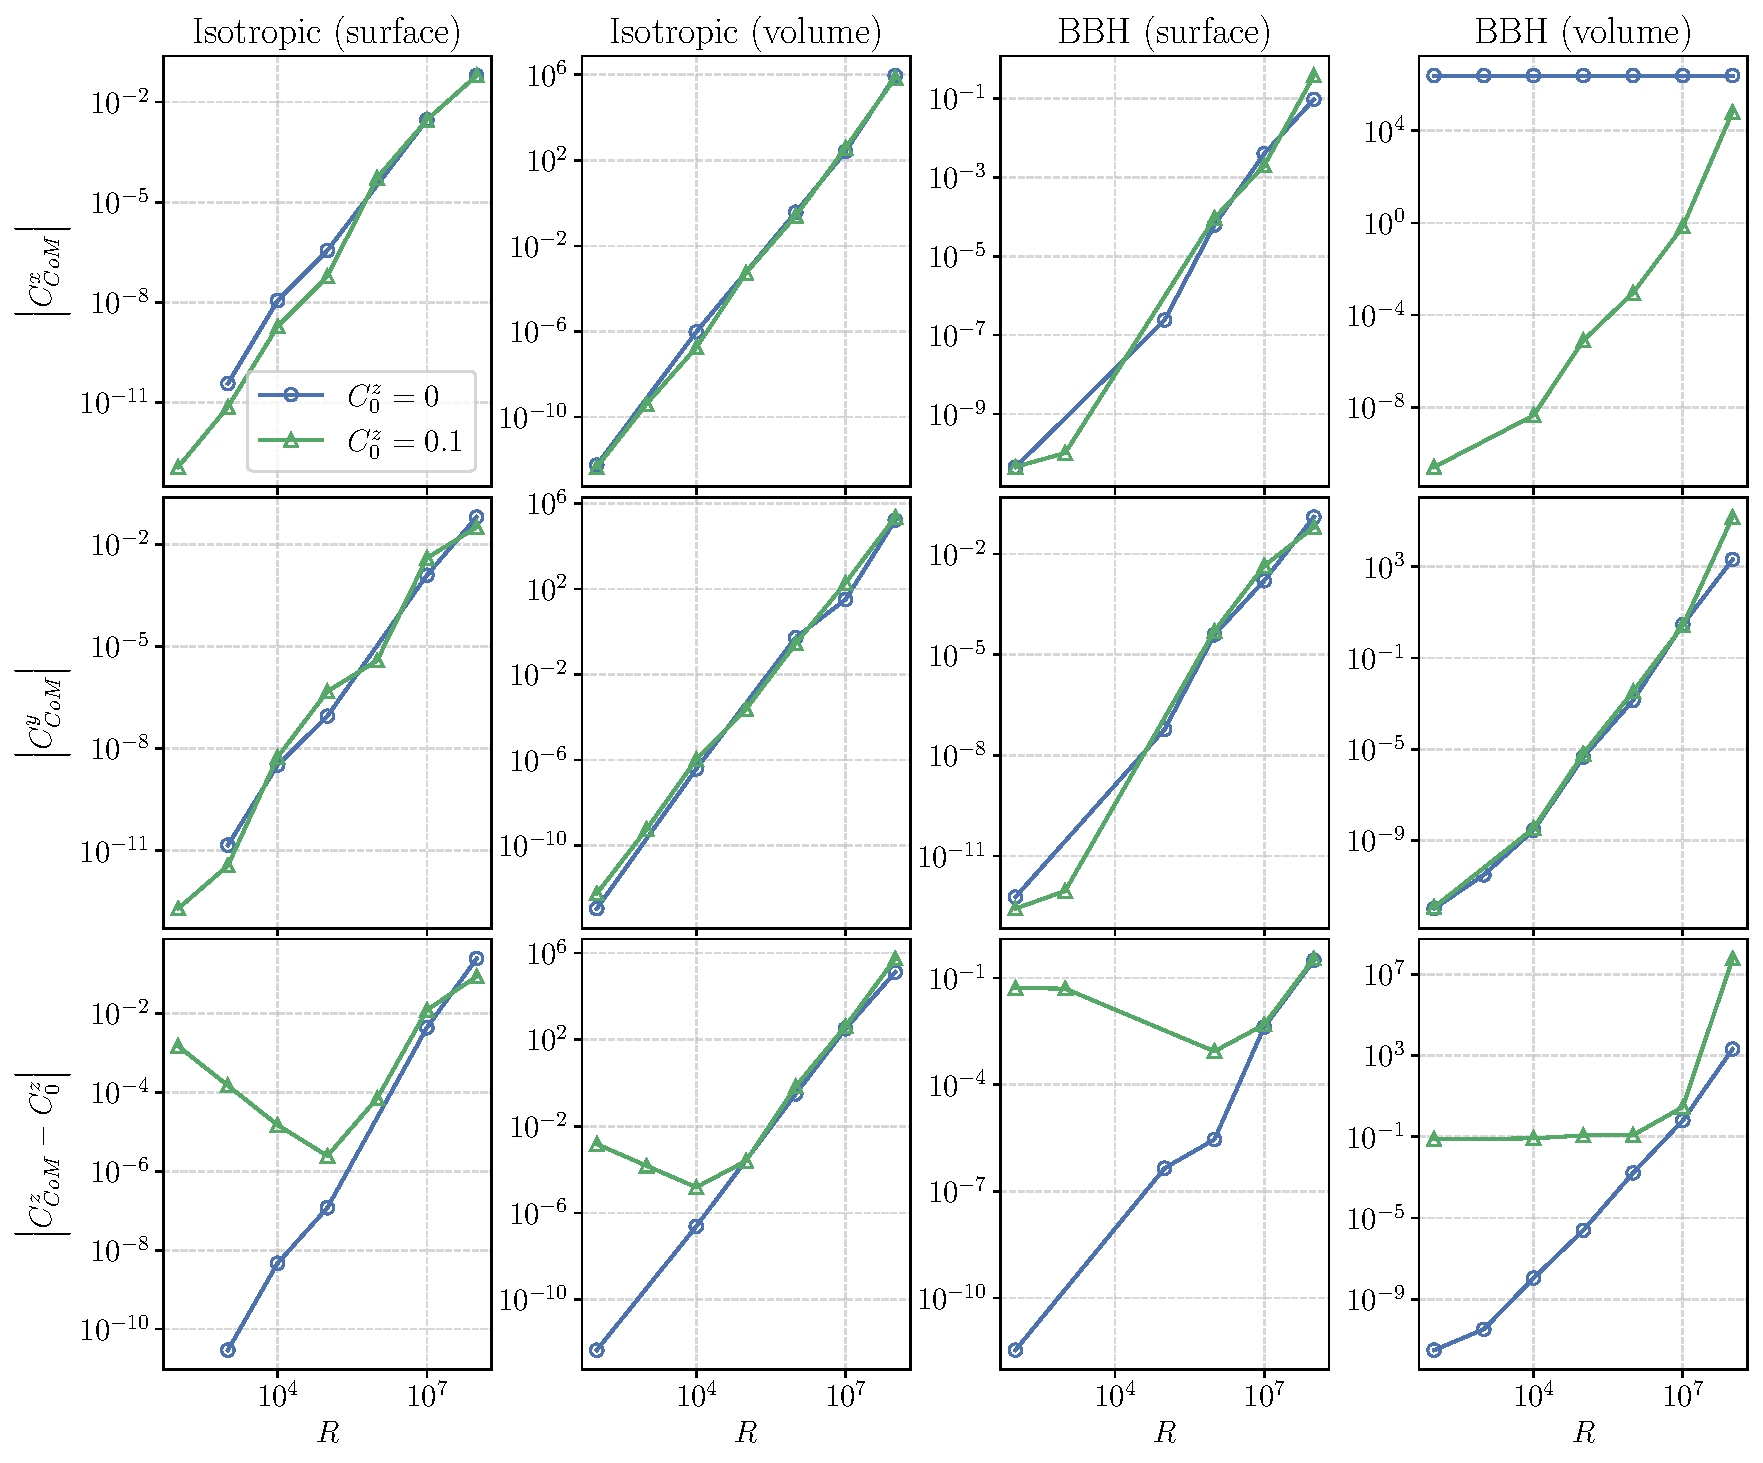
\includegraphics[width=0.85\textwidth]{../../plots/final_report/distance_convergence_CoM.pdf}
        \caption{}
      \end{figure}

      \begin{figure}
        \centering
        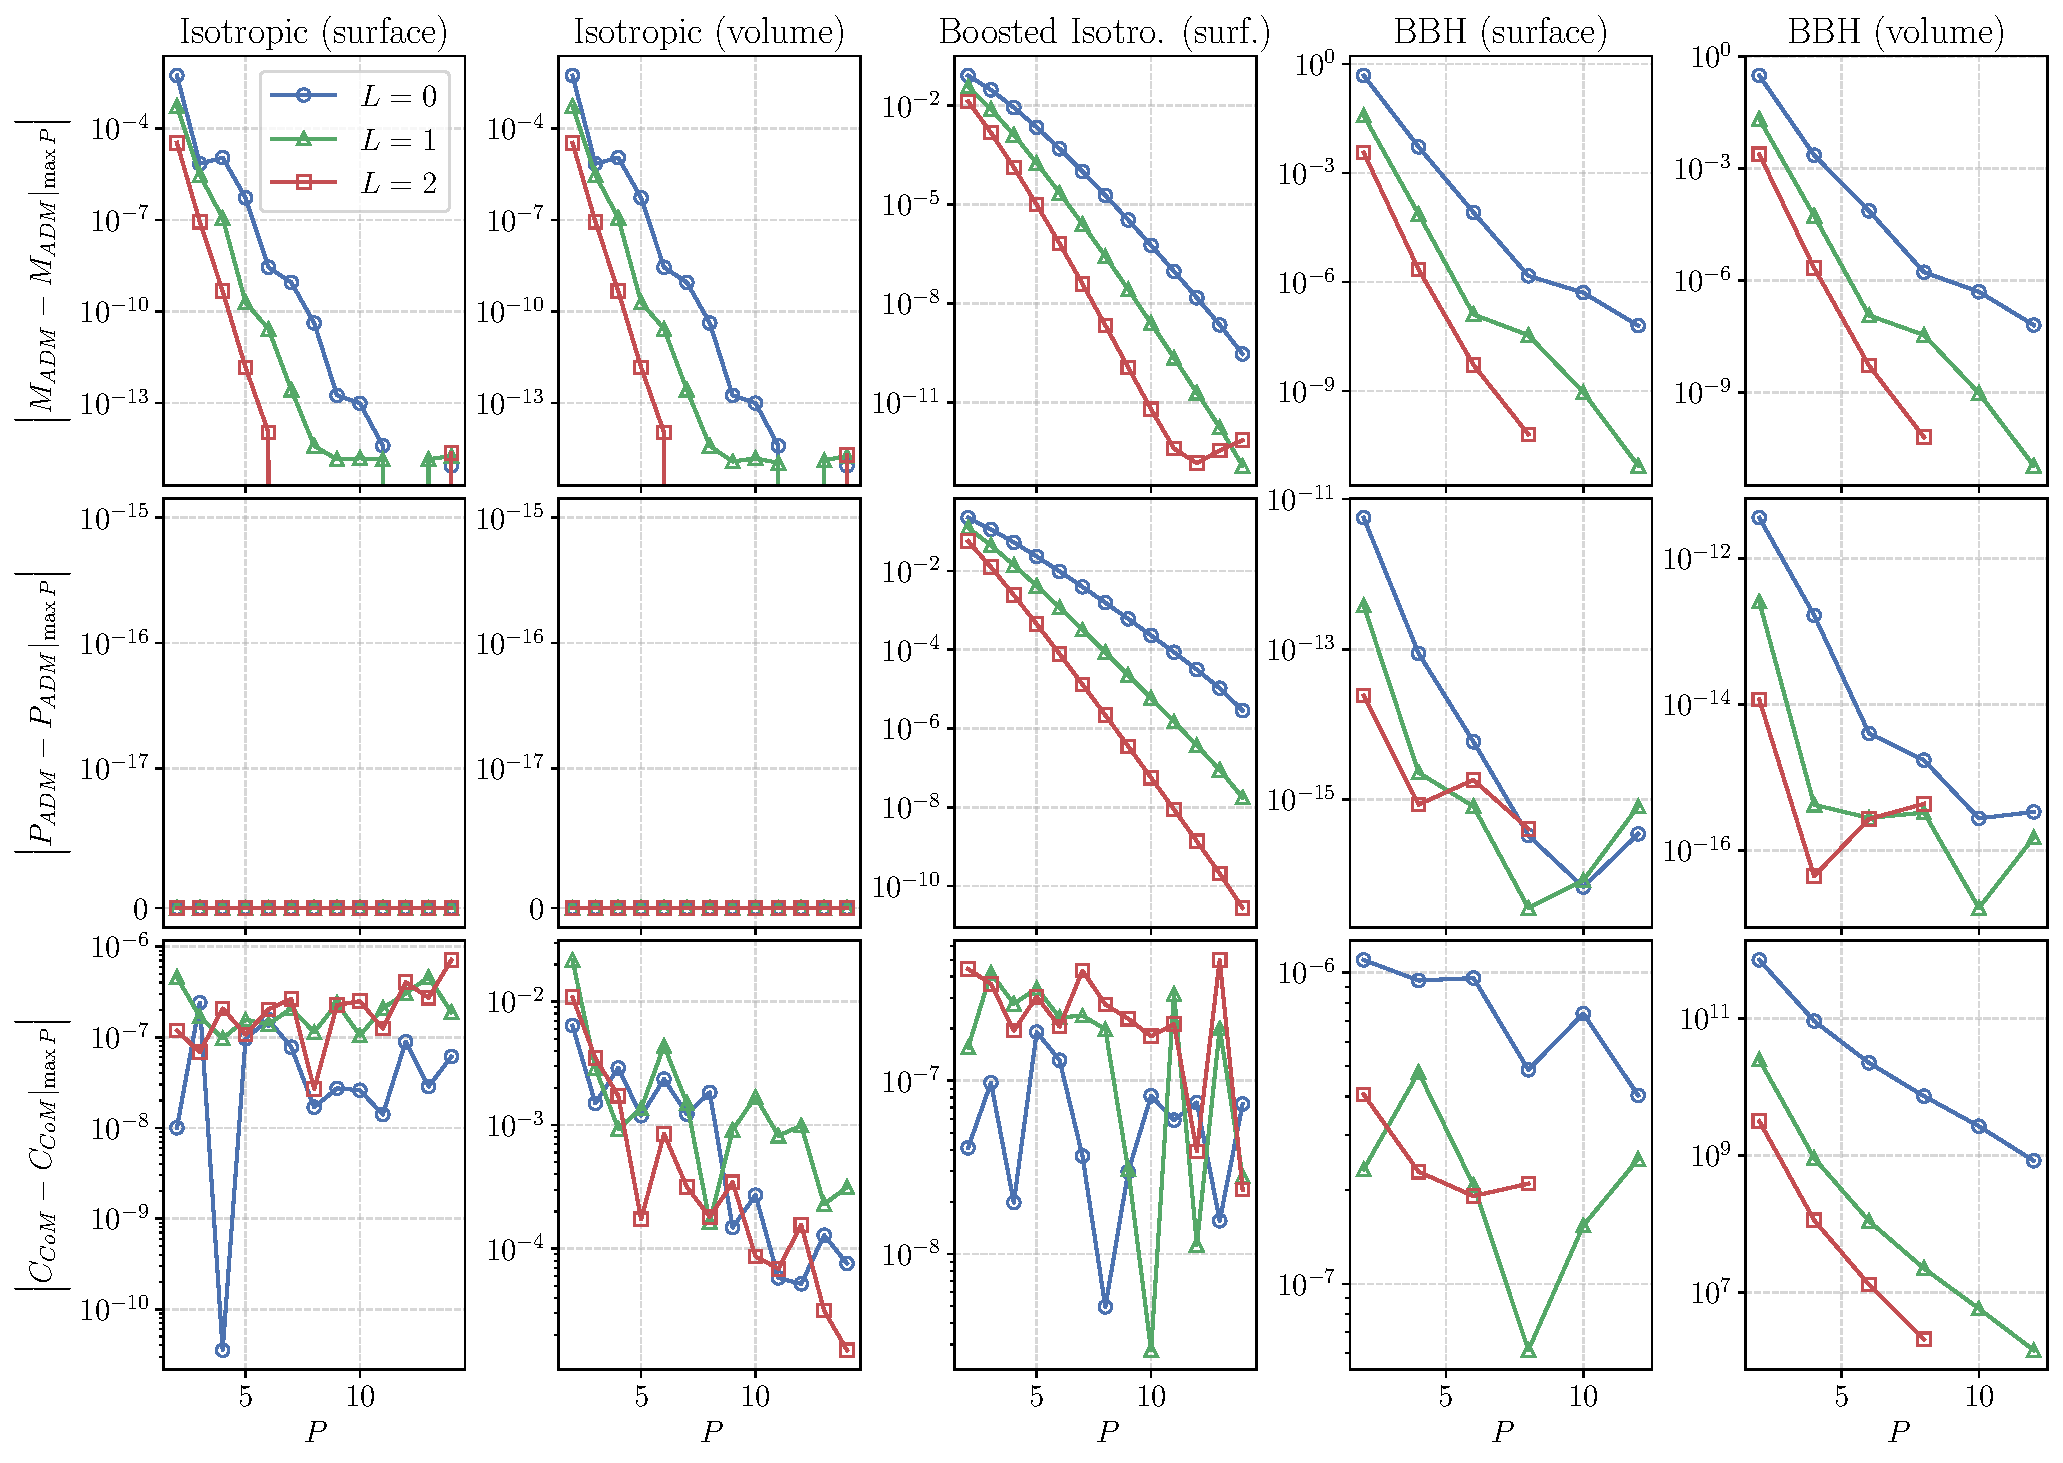
\includegraphics[width=\textwidth]{../../plots/final_report/resolution_convergence.pdf}
        \caption{}
      \end{figure}

    \subsection{Control iterations}

    \subsection{Tests over the parameter space}

  \section{Conclusion}

  \section*{Acknowledgements}

  \section*{References}

	  \printbibliography[heading=none]
  
\end{document}
